\documentclass[tikz]{standalone}

%!TEX root = main.tex

% mytikzset
\usepackage{tikz}
\usetikzlibrary{positioning,arrows,shapes,patterns}
\usetikzlibrary{decorations.pathmorphing}
\usetikzlibrary{decorations.markings}
\usetikzlibrary{decorations.pathreplacing}
\usetikzlibrary{calc}
\usetikzlibrary{patterns}
\usetikzlibrary{decorations.markings}
\usetikzlibrary{petri}

\tikzset{
  vector/.style={thick,double,draw=black, postaction={decorate},
    decoration={markings,mark=at position .6 with {\arrow[black,scale=0.4]{triangle 45}}}},
  axial/.style={thick,double,densely dashed,draw=black, postaction={decorate},
    decoration={markings,mark=at position .6 with {\arrow[black,scale=0.4]{triangle 45}}}},
  gluon/.style={decorate, draw=black,
    decoration={coil,aspect=0.3,segment length=5pt,amplitude=3pt}},
  pseudo/.style={thick, dashed, draw=black, postaction={decorate},
    decoration={markings,mark=at position .6 with {\arrow[red,scale=0.5]{triangle 45}}}},
  scalar/.style={thick,draw=black, postaction={decorate},
    decoration={markings,mark=at position .6 with {\arrow[black,scale=0.5]{triangle 45}}}},
  cut/.style={draw=black, decorate, decoration={snake, segment length=1mm, amplitude=0.2mm}}
}


\begin{document}
\nopagecolor
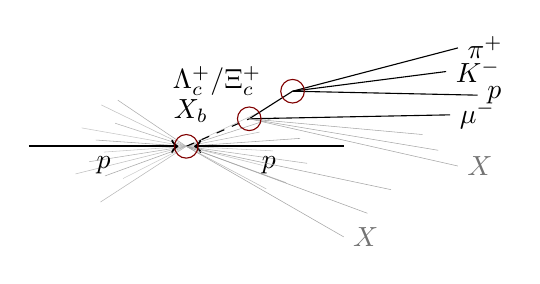
\begin{tikzpicture}[node distance=0.9cm and 1.3cm, baseline=0.9cm]
  \coordinate (pv) at (0,0);
  \coordinate (vB) at (0.8,0.35);
  \coordinate (vC) at (1.35,0.7);

  % Irregular PV activity, concentrated around the beam axis.
  \draw[very thin,black!22] (pv) -- ++(-176:1.05);
  \draw[very thin,black!30] (pv) -- ++(-171:1.25);
  \draw[very thin,black!25] (pv) -- ++(-166:1.45);
  \draw[very thin,black!35] (pv) -- ++(-160:1.10);
  \draw[very thin,black!20] (pv) -- ++(-153:0.90);
  \draw[very thin,black!28] (pv) -- ++(-147:1.30);
  \draw[very thin,black!32] (pv) -- ++(146:1.05);
  \draw[very thin,black!24] (pv) -- ++(154:1.20);
  \draw[very thin,black!30] (pv) -- ++(162:0.95);
  \draw[very thin,black!22] (pv) -- ++(170:1.35);
  \draw[very thin,black!35] (pv) -- ++(176:1.15);

  \draw[very thin,black!26] (pv) -- ++(-28:1.15);
  \draw[very thin,black!33] (pv) -- ++(-20:1.35);
  \draw[very thin,black!24] (pv) -- ++(-14:1.00);
  \draw[very thin,black!30] (pv) -- ++(-8:1.55);
  \draw[very thin,black!22] (pv) -- ++(-3:1.10);
  \draw[very thin,black!35] (pv) -- ++(4:1.45);
  \draw[very thin,black!27] (pv) -- ++(11:0.95);
  \draw[very thin,black!32] (pv) -- ++(18:1.20);
  \draw[very thin,black!24] (pv) -- ++(25:1.05);

  \draw[->,thick] (-2.0,0) -- node[below] {$p$} (-0.1,0);
  \draw[->,thick] ( 2.0,0) -- node[below] {$p$} ( 0.1,0);

  \draw[dashed] (pv) -- node[above left] {$X_b$} (vB);
  \draw (vB) -- node[above left] {$\Lambda_c^+/\Xi_c^+$} (vC);
  \draw[black] (vB) -- (3.35,0.40) node[right] {$\mu^-$};

  \draw (vC) -- (3.7,0.65) node[right] {$p$};
  \draw (vC) -- (3.3,0.95) node[right] {$K^-$};
  \draw (vC) -- (3.45,1.25) node[right] {$\pi^+$};

  \draw[very thin,black!35] (pv) -- (2.6,-0.55);
  \draw[very thin,black!35] (pv) -- (2.3,-0.85);
  \draw[very thin,black!35] (pv) -- (2.0,-1.15) node[right,black!55] {$X$};
  \draw[very thin,black!35] (vB) -- (3.0,0.15);
  \draw[very thin,black!35] (vB) -- (3.2,-0.05);
  \draw[very thin,black!35] (vB) -- (3.45,-0.25) node[right,black!55] {$X$};

  \draw[red!50!black] (pv) circle (1.5mm);
  \draw[red!50!black] (vB) circle (1.5mm);
  \draw[red!50!black] (vC) circle (1.5mm);
\end{tikzpicture}
\end{document}
